\pagenumbering{gobble}
~
\cleardoublepage
\begin{center}
~
\vskip 10em
``The world wasn't destroyed. There was no great catastrophe. Nothing in particular went wrong. The trains just stopped running.''

- Nathaniel Ford 5/10/12
\end{center}

\setcounter{page}{1}
\pagebreak
\pagenumbering{roman}
\setcounter{page}{2}

\jumpHeadline{Adam}
\textbf{Character:} Oliver Langdon\\
\textbf{Nickname: }L[a-z]*	\\
\textbf{Class: }Citizen	\\
\textbf{Serial Number: }1195725475	

``While on duty, Oliver slouches and keeps a day's stubble growth on his face.  His mid-brown hair looks to be cut by someone with apathetic scissors.  His uniform conceals the surgical repair of his bad knee, but nothing can hide his lopsided limp.  Though he has a poor complexion and a bad attitude towards authority, he is quite likeable and forms friends quickly - even among those below his social class.  Though he never speaks of Transit Minor, a shadow of past trauma hovers near him, visible to those who are sensitive to such nuances.

When in the company of his peers outside of the Authority, Oliver's posture, outward politeness, and personal upkeep improve dramatically, but his bitterness and anger at those in positions of power still erupt sometimes.''

\vskip 5em

\jumpHeadline{Ion}
\textbf{Character:} Jonah Gemayel (Timon)		\\
\textbf{Class: }National (Franchise)	\\
\textbf{Serial Number:} 4018675308	

``Dark, mid-length wavy hair, dark eyes.  Usually with a small amount of stubble, neither well-shaven (the mark of the wealthy) nor so long as to be unkempt.  Average height, fairly fit. �He dresses practically, the uniform of the TA being joined by the packs and pragmatic satchels of a street medic.  Jonah appears to be relaxed most of the time, with a cheerful but mild attitude, and a small but constant smile.  That other people tend to see him as friendly but not terribly notable, is a testament to his nearly constant attention to maintain this demeanor at all costs.  The facade rarely cracks.  When it does the tension in his eyes that flickers into view is momentary and so out of place it is easily dismissed.''
 
 \pagebreak
 \jumpHeadline{Rebecca}
\textbf{Character:} Jaya Parvadi	\\
\textbf{Nickname: }Patches	\\
\textbf{Class:} Franchise\\
\textbf{Serial Number:}	1195725475	

``Red rimmed eyes, heavily lidded under heavy brows. A gaunt face atop an equally tall, gaunt form. What little body fat she has is not worn well. Tattoos crawl over her dark skin. They curl below her lips, spot her limbs, and disappear down the cuffs and collar of her worn Transit Authority uniform. Chemical stains are visible on fingers and teeth that flash in grins or grimaces every time she takes another drag on some hand rolled cigarette.''

\vskip 10em

\jumpHeadline{Suko}
\textbf{Character:} Hayley	\\	
\textbf{Class:} Incorporated	\\
\textbf{Serial Number:} 2460124601	

``Appears to be in her late teens at first glance, but is probably in her early 20's.  Stunningly good looking, Hayley has huge pale blue-grey eyes, a flawless golden complexion and absolutely symmetrical features.  There is a certain doll-like blankness to her expression.  Her glossy black hair is cut in a practical short cropped style that only serves to emphasize her elegant bone structure.  Her figure is tall, leggy and nicely proportioned.  She looks healthy, and only slightly less nourished and well fed than a Citizen.  Certainly better than most Indentured.  She is toned and fit, and moves gracefully like a dancer.  She has excellent posture, always.  You have never seen her slouch or sprawl.  For those who notice such things, she does not act like someone who is really aware of how their appearance impacts other people.  She certainly does not purposely solicit that type of attention.''

\pagebreak

\begin{center}
~
\vskip 7em
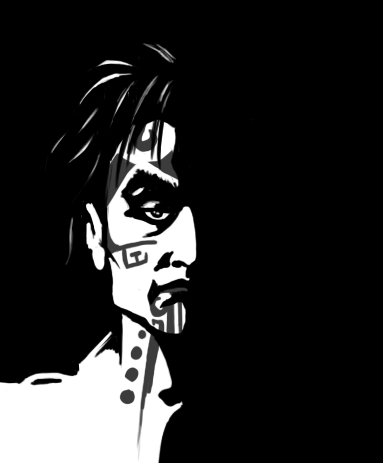
\includegraphics[width=5cm]{img/book1_jaya_shadow.png}
\end{center}

\pagebreak
\pagenumbering{arabic}
\setcounter{page}{7}